\chapter{Layer 2}
It's the layer responsible of sending packets over the network. As it will be explained in Chapter \ref{layer3} , Layer 3 network disappeared and all local area network are supported by Layer 2. Hence routing isn't needed in the network anymore.\\
When a smartphone connect to a network, uses a Point to Point Layer 2 connection using LTE/4G/5G, and it's connected to Local Network Area (LAN) using WiFi. Layer 2 supports protocols HDLC, PPP(Point to Point Protocol) in Point to Point connections and Ethernet(IEEE 802.3 802.11) in LAN (Local Area Networks).\\
Hence Internet Packet passes only through two types of networks: Point to Point link or Local Area Networks.
\begin{figure}[h]
\centering
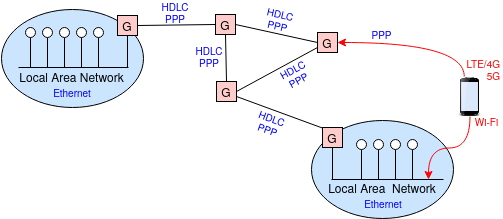
\includegraphics[scale=0.4]{Images/Layer2/layer2}
\caption{\footnotesize{Nowadays L2 connections.}}\label{layer2}
\end{figure}

\section{Ethernet}
In Ethern protocol, there was a coaxiale cable, long about 1.5 km, on which host interconnect (Figure \ref{ethernet}). All the hosts electrically shared a bus. In the past hosts ethernet interfaces were connected through a vampire tap junction but now, they are connect to cable using a T-junction (see Figure \ref{vampire_tap} and Figure \ref{t_junction}). The difference between them is that the first one connects electrically to the cable (connecting it to a cable cut) and the second one is used only in ethernet cables that are physically composed by different cable (segments) and the T-junction is put at intersection of two segments.\\
The protocol supports Carriege Sense Multiple Access Collision Detection (CSMA/CD), used for coordination between hosts, that it's composed by two strategies:
\begin{itemize}
\item{\textbf{Carrier sense}\\
An host can't speak while anyone else is speaking}
\item{\textbf{Collision detection}\\
the protocol resolves conflicts raised during the contention time. Contention time is the time in which people, that respect first rules, can also go in conflict starting talking together at the same moment.}
\end{itemize}
\begin{figure}[h]
\centering
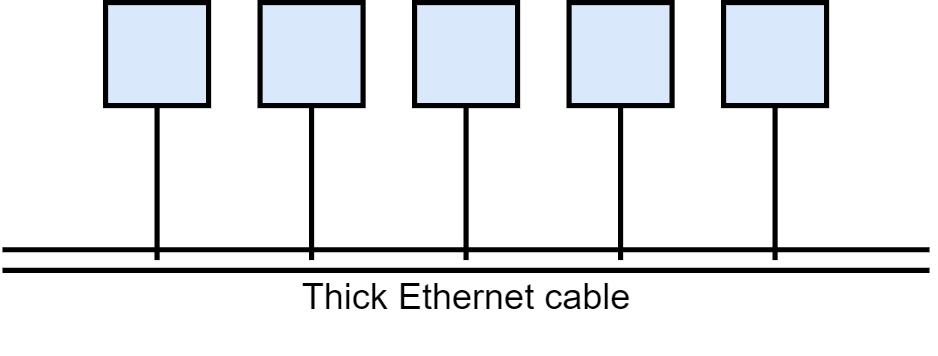
\includegraphics[scale=0.3]{Images/Layer2/ethernet}
\caption{\footnotesize{Ethernet.}}\label{ethernet}
\end{figure}
\begin{figure}[h]
\centering
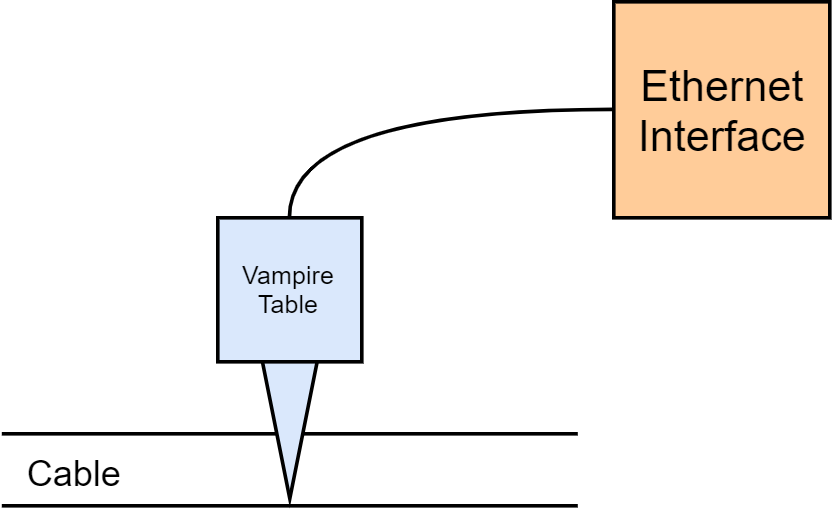
\includegraphics[scale=0.3]{Images/Layer2/vampire_tap}
\caption{\footnotesize{Vampire tap.}}\label{vampire_tap}
\end{figure}
\begin{figure}[h]
\centering
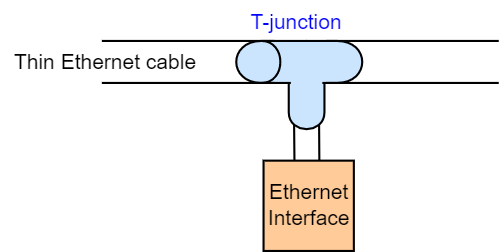
\includegraphics[scale=0.5]{Images/Layer2/t_junction}
\caption{\footnotesize{T-junction.}}\label{t_junction}
\end{figure}
In Figure \ref{collision}, $N_B$ detects the collision only when the packet from $N_A$, arrives to $N_B$, after the collision with the packet sent by $N_A$.\\
\begin{figure}[h]
\centering
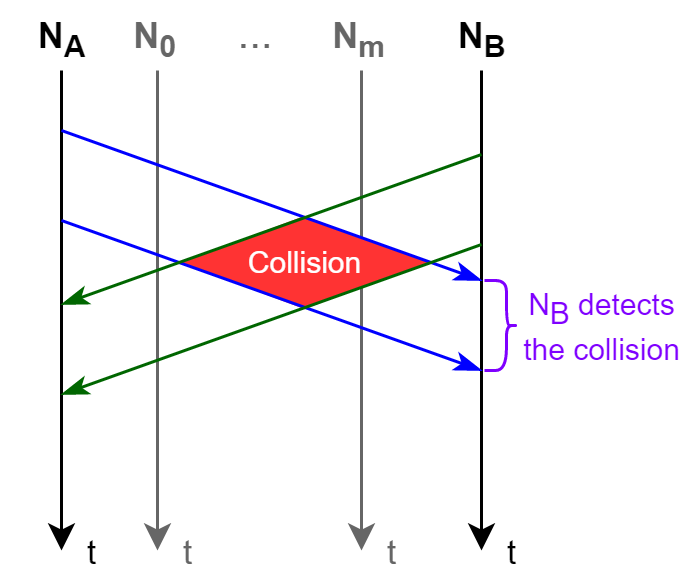
\includegraphics[scale=0.35]{Images/Layer2/collision}
\caption{\footnotesize{Collision detection.}}\label{collision}
\end{figure}
The \textbf{propagation time (pt)} is the time between the moment in which the host sends the message and  the one in which the message arrives to remote host.
This time is computed w.r.t. value of light velocity(ideal velocity of packets in Internet) and the absolute distance between the two hosts, that are talking each other.
$$propagation\;time\;(pt)\;=\; \frac{absolute\;distance}{light\;velocity}$$
Considering that the absolute distance is about km ($10^3$ m), the value of the light velocity is $10^8$ m/s and the bandwith is about $10^7$ bit/sec, we obtain that we can transmitt $10^2 bit$. Hence we could transmit about 10$\div$100 bytes, but then the number of bytes was standardized to 64 bytes.
\begin{figure}[H]
\centering
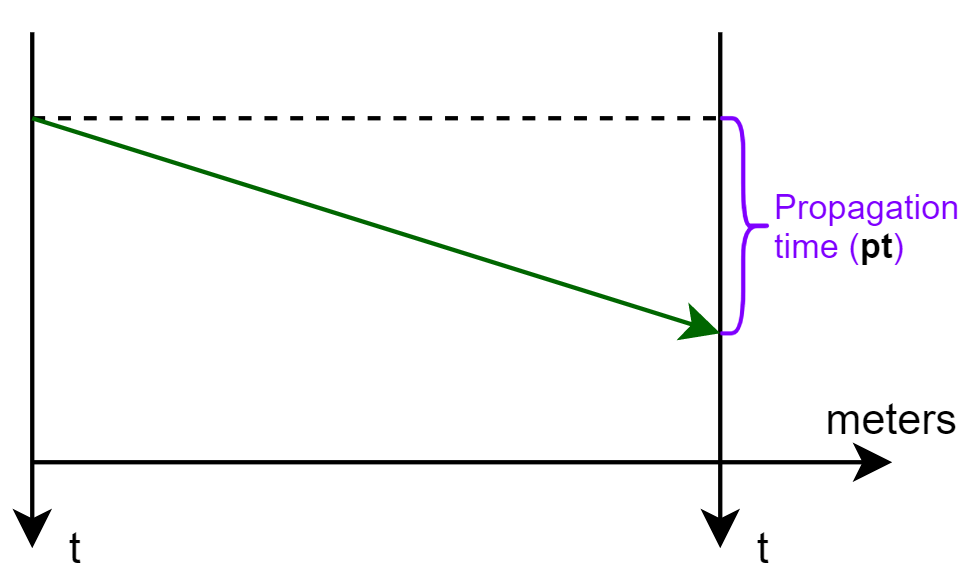
\includegraphics[scale=0.3]{Images/Layer2/pt}
\caption{\footnotesize{Propagation time.}}\label{pt}
\end{figure}
To avoid the collision, when $N_B$ detect the collision, it waits a ranom time to send again the lost previous packet (Figure \ref{collision_avoid}). The random time is defined as follows:
$$random\;time=rand()*2*pt$$
If there is another collision during this period, the random value \textit{rand()} increases the range in which we can generate a random value. This ranges are defined through this \textit{exponential backoff} sequence:
\begin{table}[h]
\centering \footnotesize
\begin{tabular}{rl}
\textbf{1)} & {$[0,1]$}\\
\textbf{2)} & {$[0,3]$}\\
\textbf{3)} & {$[0,7]$}\\
\multicolumn{2}{c}{...}\\
\textbf{4)} & {$[0,2^n-1]$}\\
\end{tabular}
\end{table}
\begin{figure}[H]
\centering
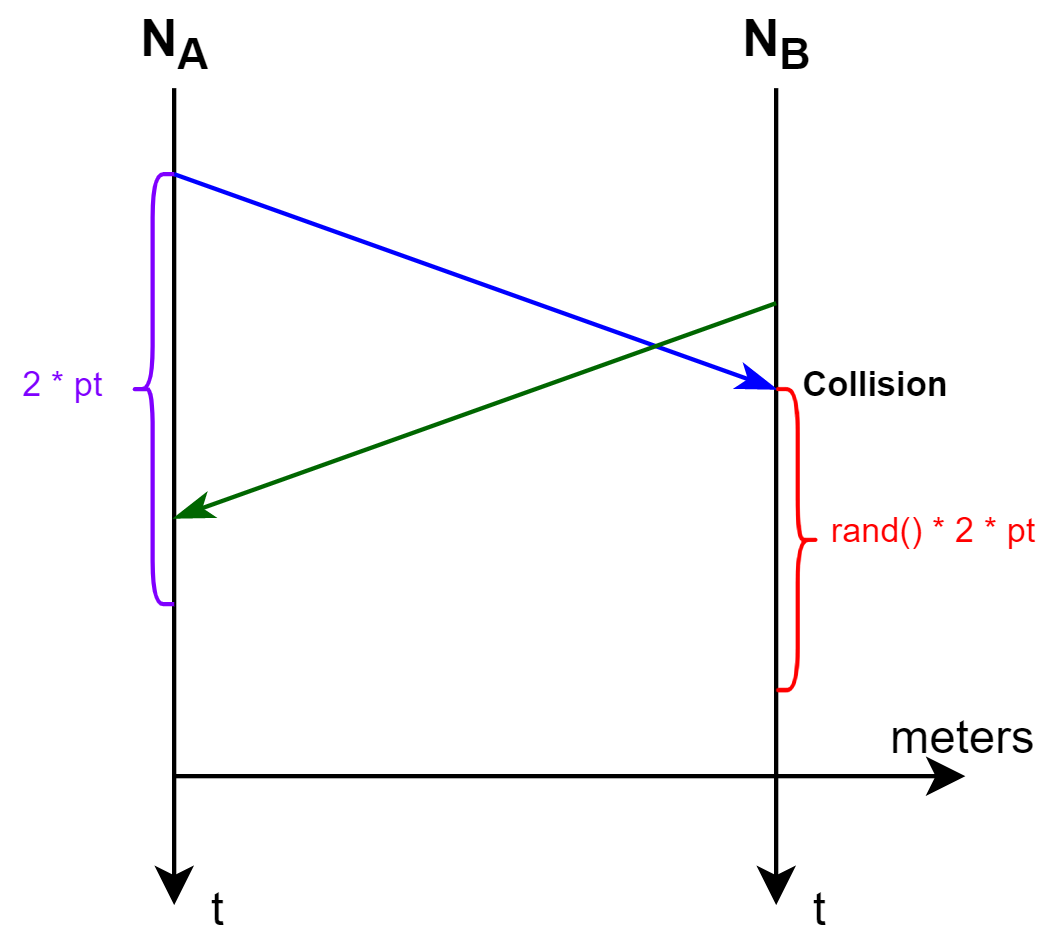
\includegraphics[scale=0.3]{Images/Layer2/collision_avoid}
\caption{\footnotesize{Collision avoid.}}\label{collision_avoid}
\end{figure}

\subsection{Ethernet frame}
\begin{figure}[H]
\centering
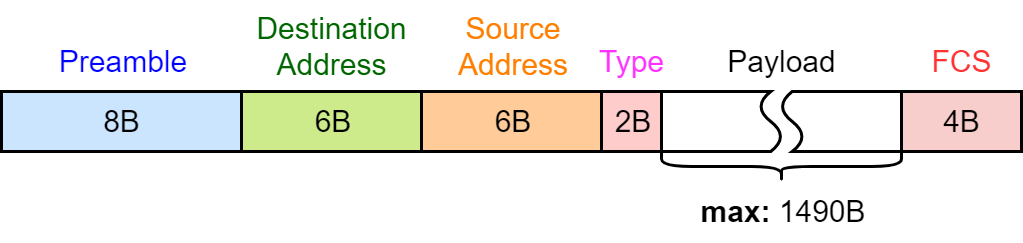
\includegraphics[scale=0.3]{Images/Layer2/layer2_message}
\caption{\footnotesize{Ethernet packet.}}\label{layer2_message}
\end{figure}
\begin{itemize}
\item{\textbf{Preamble}\\
synchronization signal \textit{10101010...1010}\textbf{011} where the last three bits are called \textbf{SFD()}.
}
\item{\textbf{Destination address \& Source address}\\
MAC (Medium Access Control) addresses, that are Hardware identifiers (broadcast= \textbf{ff:ff:ff:ff:ff:ff}).  
}
\item{\textbf{Type}\\
type of ethernet frame used.
}
\item{\textbf{Payload}\\
payload of the ethernet frame.
}
\item{\textbf{FCS}\\
Frame check sequence (FCS) is a CRC that allows detection of corrupted data within the entire frame as received on the receiver side.
}
\end{itemize}

\subsection{Hub and switches}
\begin{figure}[H]
\centering
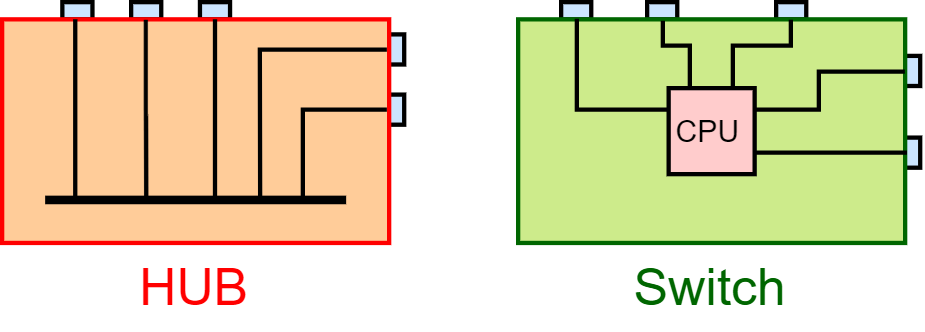
\includegraphics[scale=0.3]{Images/Layer2/hub_vs_switch}
\caption{\footnotesize{Hub and switches.}}\label{hub_vs_switch}
\end{figure}
There two main types of devices, that uses ethernet and creates LANs, are (Figure \ref{hub_vs_switch}):
\begin{itemize}
\item{\textbf{Hub}
\begin{figure}[H]
\centering
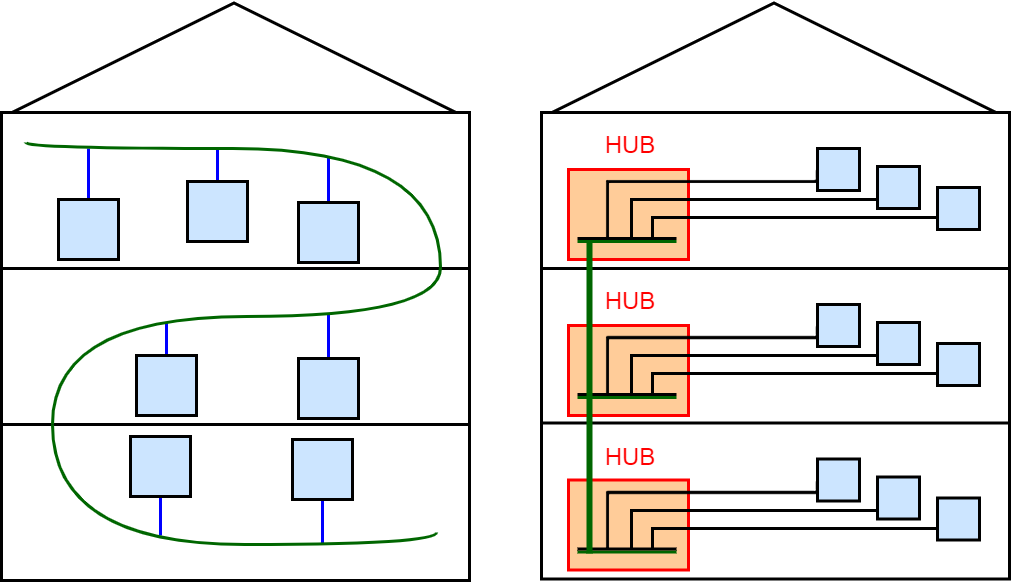
\includegraphics[scale=0.3]{Images/Layer2/cable_vs_hub}
\caption{\footnotesize{Cabled LAN vs LAN with hubs.}}\label{cable_vs_hub}
\end{figure}
\begin{itemize}
\item{All the nodes, connected to the hub, receive all packets sent by another node but only destination node considers it. The other ones discard them.}
\item{Broadcast is very efficient.}
\item{There is Collision.}
\item{Network security level is very low.}
\end{itemize}
}
\item{\textbf{Switch}
\begin{figure}[H]
\centering
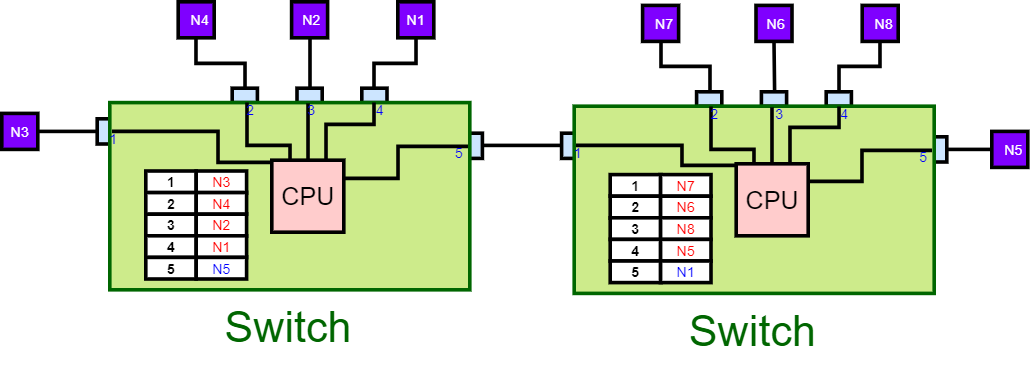
\includegraphics[scale=0.5]{Images/Layer2/switch}
\caption{\footnotesize{Switch connection.}}\label{switch}
\end{figure}
\begin{itemize}
\item{Only the destination node can see the packets sent by another node to it.}
\item{There aren't collision.}
\item{Broadcast is supported.}
\end{itemize}
In the example of Figure \ref{bandwidth_switch}, there is an aggregate bandwitch of 200 Mbps on a 100 Mbps network.
\begin{figure}[H]
\centering
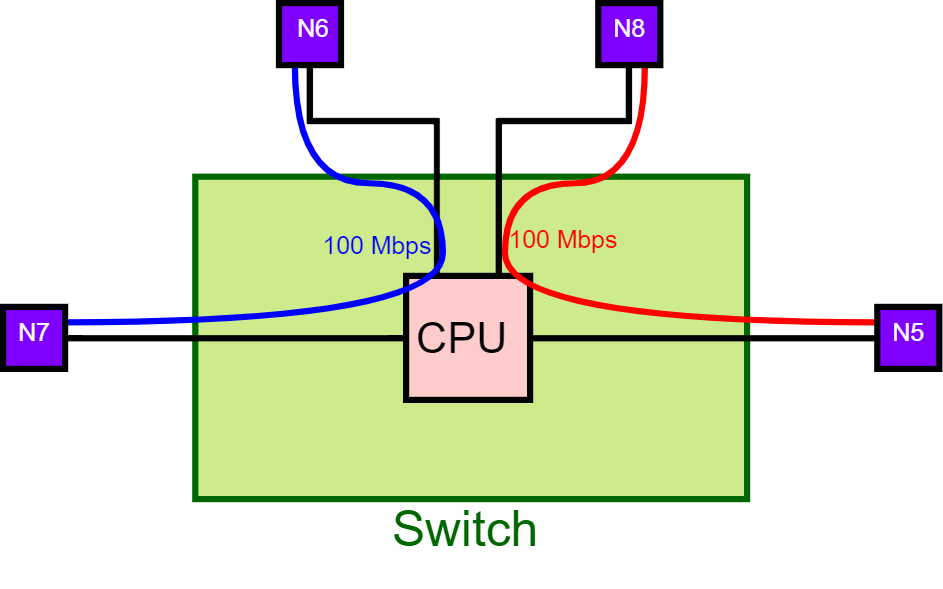
\includegraphics[scale=0.4]{Images/Layer2/bandwidth_switch}
\caption{\footnotesize{Bandwidth switching.}}\label{bandwidth_switch}
\end{figure}
}
\end{itemize}

\subsection{Virtual LAN (VLAN)}
Using switches, we can also logical create subnetworks of the hosts connected to the switch. For security reason, the access, to other subnetworks of the hosts connected to the hub, is usually managed through gateways connected to particular ports of the switch. Hence a packet, sent from a virtual network to another one, is sent to that ports to be able reach the final destination.
\begin{figure}[H]
\centering
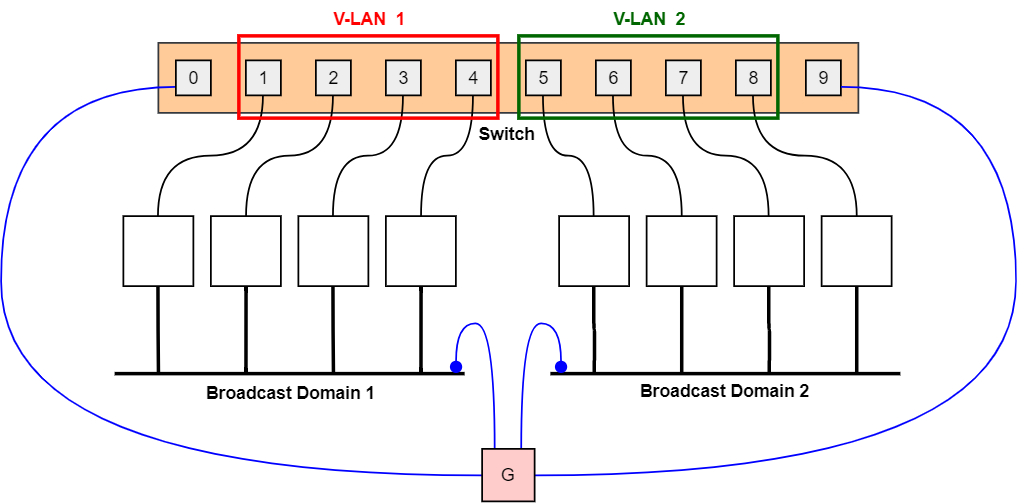
\includegraphics[scale=0.4]{Images/Layer2/vlan}
\caption{\footnotesize{VLANs.}}\label{vlan}
\end{figure}
It is also possible to create a VLAN over 2 different switches (Figure \ref{tunnel}). The connection between the two switches is done by adding an Layer-2 or Layer-3 connection. In the second case the connection is called \textit{Lan Emulation Tunneling (VPN)}.
\begin{figure}[H]
\centering
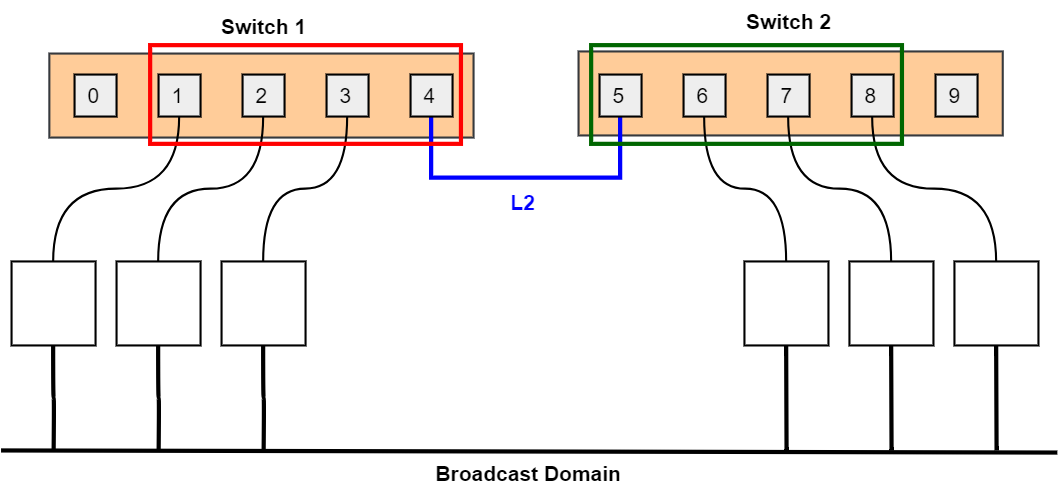
\includegraphics[scale=0.35]{Images/Layer2/tunnel_l2}
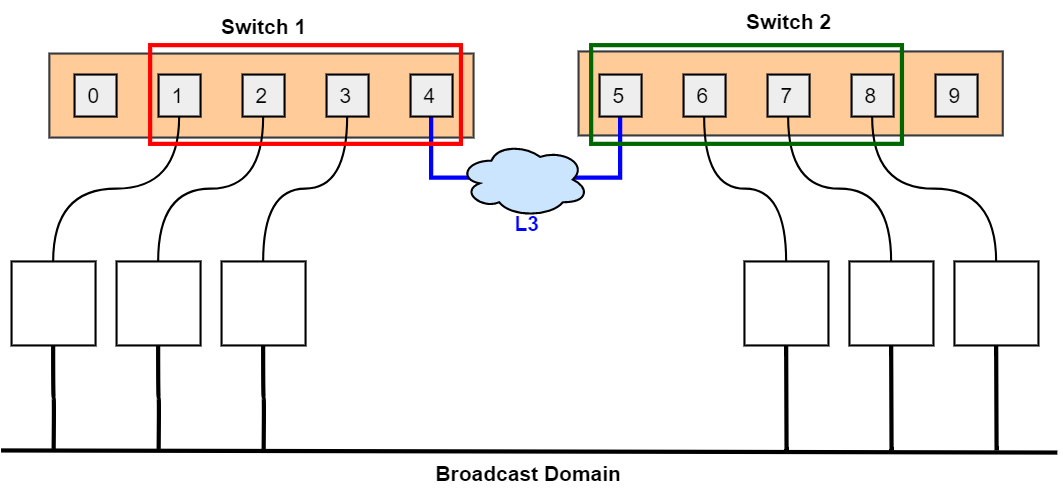
\includegraphics[scale=0.35]{Images/Layer2/tunnel_l3}
\caption{\footnotesize{VLAN over two switches.}}\label{tunnel}
\end{figure}

\subsection{Address Resolution Protocol (ARP)}
Using the Ethernet protocol and sending an Internet Protocol packet, the sender needs to know MAC address of remote node. To resolve the IP address of the remote host, we use the DNS protocol. After the IP address is found, we need to resolve the IP address of the destination host into the MAC address of corresponding machine, using the \textbf{Address Resolution Protocol (ARP)}.\\
This method works as follows (Figure \ref{ARP}):
\begin{center}
\begin{tabular}{c}
\begin{lstlisting}[linewidth=410pt, basicstyle=\footnotesize\sffamily,]
if( (IP_dest & netmask_src) == (IP_src & netmask_src))
{
		/*
		The source and the destination are in the same network (LAN)
		The answer is sent in broadcast to all the hosts in the network, specifying
		the IP_dest and the host that has the specific IP_dest, replies with its
		MAC_dest
		
		Then there will be a new packet, sent to [IP_dest, MAC_dest] machine
		(example of this packet in the Figure 6.15)	
		*/
}
else
{
		/*
		The source and the destination are in different networks (LANs)
		The answer is sent in broadcast, from H_src, asking for the MAC_gat of
		the host in the LAN with with IP_gat 

		Then knowing it, it will be sent a new packet to the specific gateway
		host MAC_host but specyfing IP_dest
		(example of this packet in the Figure 6.15)	
		*/
} 
\end{lstlisting}
\end{tabular}
\end{center}
\begin{figure}[H]
\centering
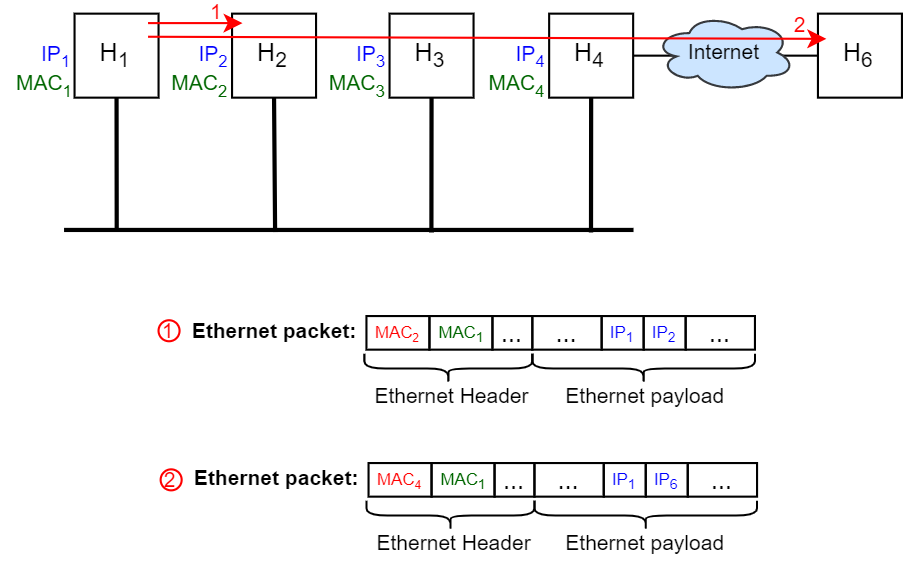
\includegraphics[scale=0.45]{Images/Layer2/ARP}
\caption{\footnotesize{ARP.}}\label{ARP}
\end{figure}